\paragraph{Visualizzazione pagina profilo}

\subparagraph{Pagina profilo personale}

\label{Pagina profilo personale}

\begin{figure}[ht]
	\centering
	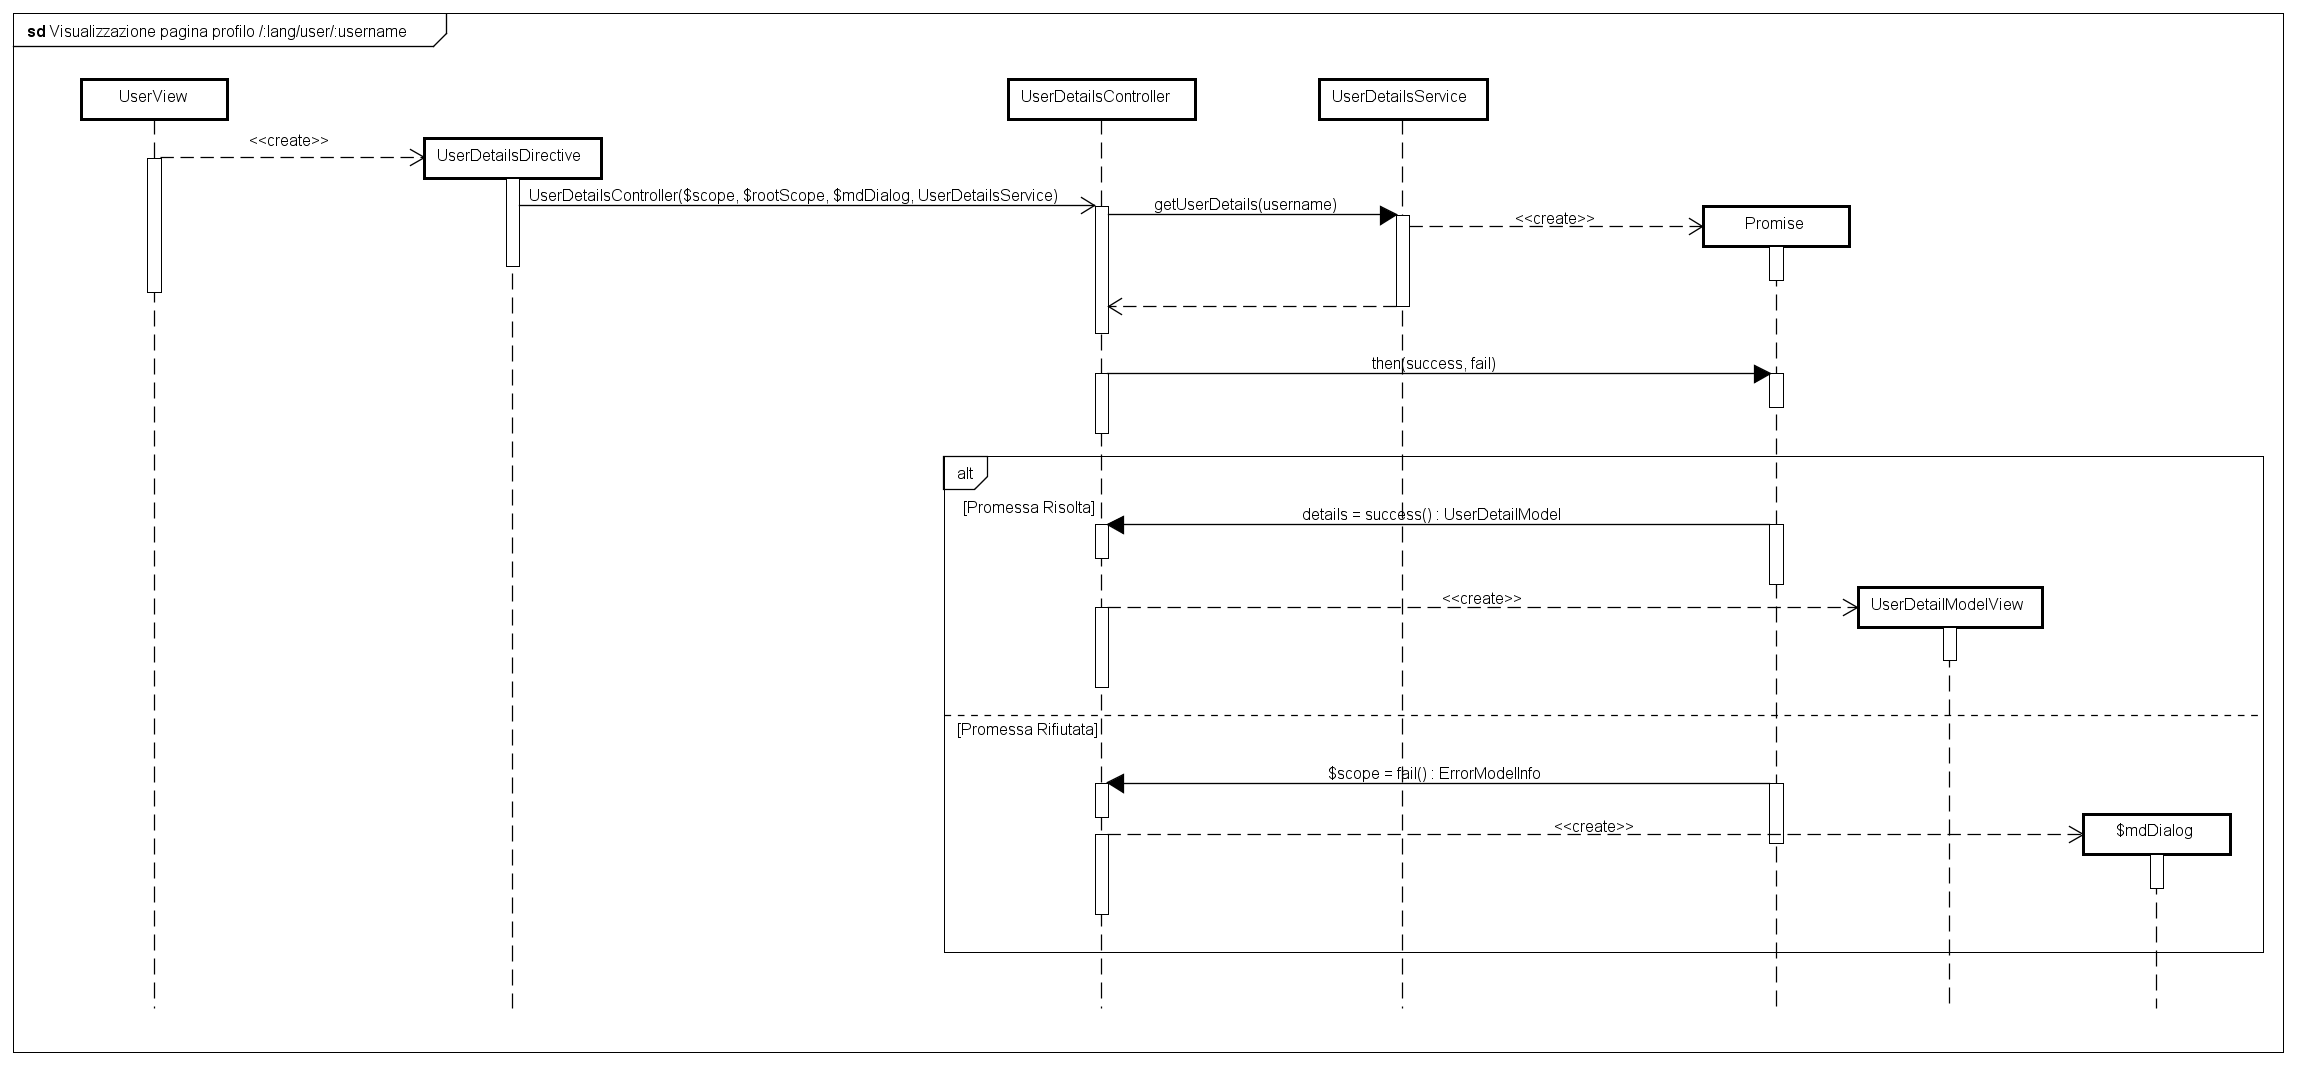
\includegraphics[scale=0.25,keepaspectratio]{UML/DiagrammiDiSequenza/Front-end/UserPage.png}
	\caption{Pagina profilo personale}
\end{figure} \FloatBarrier

Con tre chiamate asincrone dai corrispettivi controller, le directive \texttt{StatisticsDirective}, \texttt{UserDetailsDirective}, \texttt{QuestionnaireDetailsDirective} e \texttt{QuestionnaireDetailsDoneDirective} vengono popolate e mostrate all'utente. 
In questo diagramma di sequenza viene mostrato solamente il processo di creazione e visualizzazione della directive \texttt{UserDetailsDirective} poiché il procedimento per tutte le altre directive è simile.

\subparagraph{Pagina profilo altri utenti}

La sequenza di operazioni necessaria per visualizzare una pagina profilo di un altro utente è del tutto simile a quella del profilo personale, ad eccezion fatta per la sezione dei questionari. 
